\section{Gantt Chart} \label{sec:appF}
The current critical path starts with ordering and receiving parts, until this is done building cannot take place. The key components are the pump, valves, tubing, fittings and Arduino. Once orders have been received building can take place and then testing can begin. All remaining tests require some degree of building to be completed. Certain tests such as Test 17 in Table \ref{tab:samples-condensation-test} require the entire pneumatic system to be completed and others such as Test 2 in Table \ref{tab:data-coll-test} require just the electronics and software.
\subsection{Gantt Chart (1/2)}
\begin{figure}[H]
    \begin{align*}
        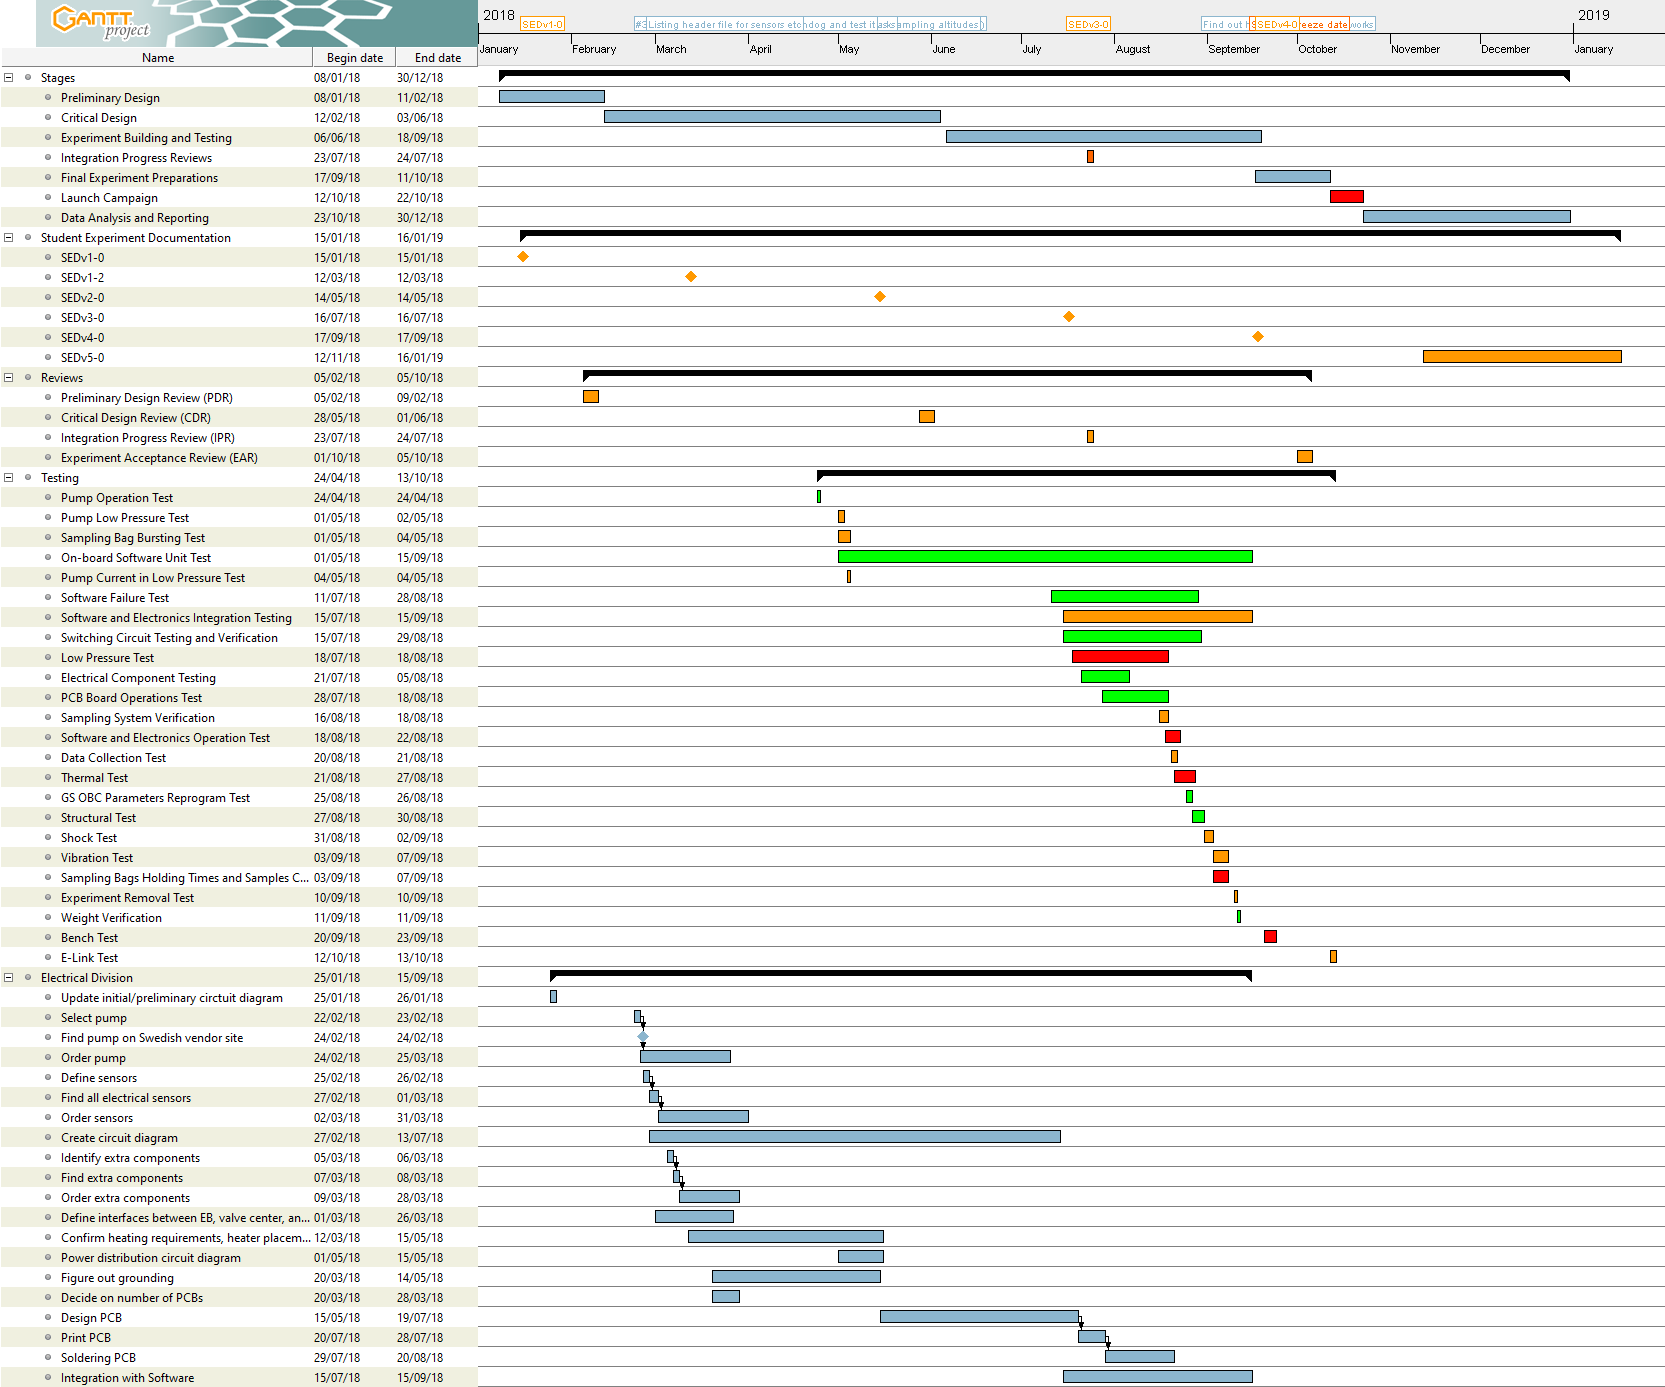
\includegraphics[width=1\textwidth, height=0.80\textheight]{appendix/img/gantt-chart/gantt-chart-part-one.png}
    \end{align*}
    \caption{Gantt Chart (1/2).}
    \label{fig:gantt-chart-1}
\end{figure}

\subsection{Gantt Chart (2/2)}

\begin{figure}[H]
    \begin{align*}
        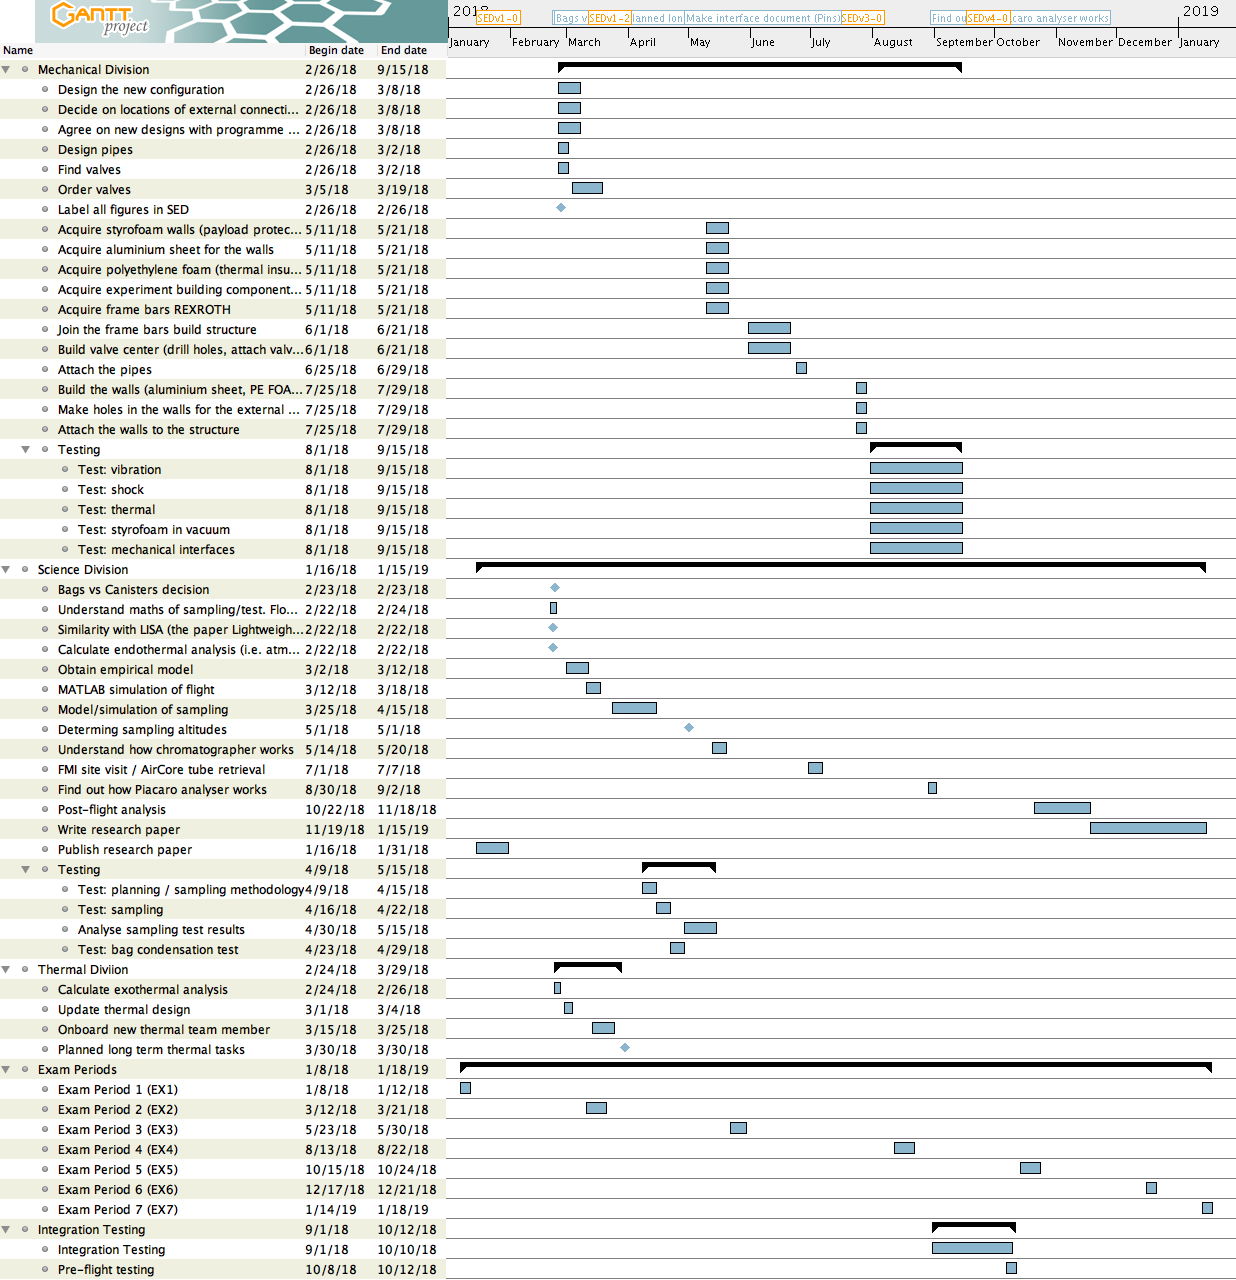
\includegraphics[width=1\textwidth, height=0.85\textheight]{appendix/img/gantt-chart/old-gantt-chart-2.png}
    \end{align*}
    \caption{Gantt Chart (2/2).}
    \label{fig:gantt-chart-2}
\end{figure}

By comparing the team availability in Appendix \ref{sec:appD} to the Gantt chart it can be seen that across the summer there is lower team availability. In this time frame there are two periods with particularly low team availability; The early summer and early August. The work has been planned so that the critical work will be completed in the periods with higher availability. In the event that the work takes longer than expected the question marks can become green.